\section{Integer Programming}

This chapter only covers integer \textit{linear} programming, mind you.

\subsection{Motivation}

\subsection{Why is this any harder?}

We've just been through the \textsc{Simplex} algorithm, and we're exhausted. How can we
possibly dedicate a whole chapter to something that is all but identical to what
we've just been through?\\

This is why:

%\begin{figure}[ht]
%\begin{minipage}[b]{0.45\linewidth}
%\centering
%\includegraphics[scale=0.2]{images/valve.jpg}
%\caption*{Linear programming}
%\label{fig:figure1}
%\end{minipage}
%%\hspace{0.5cm}
%%\begin{minipage}[b]{0.45\linewidth}
%\marginnote{\textit{This metaphor is gonna suck...}}[-0.5cm]
%\centering
%\includegraphics[scale=0.2]{images/valve.jpg}
%\caption*{Integer programming}
%\label{fig:figure2}
%\end{minipage}
%\end{figure}

Well, not quite. Think of our decision variables $x \in \mathcal{R}^n$ as valves.
\marginnote{\textit{This is what you meant by the buttons. We have to go through all
these toggle combinations!}}[-0.5cm]
We can increase or decrease them to our \textsc{Simplex} method's heart's desire, and as
long as we're in the feasible simplex, everything is jolly. However, if we impose
the integer constraint $x \in \mathcal{B}^n$, then our feasible region suddenly
looks quite "spotty", meaning that only integer solutions are feasible. 

In fact, it's \np-hard! % Add reference to Karp's 21 NP-hard problems

The following section describes how we can solve integer programs, in part by
linear programming!

\subsection{Computational Complexity}

\subsection{Bounds}

Here I will briefly go through a selection of relaxations. It assumes that you
now what \hyperref[sec:duality]{duality} is!

Consider two programs:

\begin{equation}
RP: w = \mathrm{max}\: \{f(x)\:|\:x\in T \subseteq \mathcal{R}^n\}
\end{equation}

\begin{equation}
IP: z = \mathrm{max}\: \{c(x)\:|\:x\in X \subseteq \mathcal{R}^n\}
\end{equation}

Then $RP$ is a relaxation of $IP$ if:

\begin{equation}
\begin{split}
\text{\textbf{i)}\hspace{0.5cm}}  & X \subseteq T\\
\text{\textbf{ii)}\hspace{0.5cm}} & f(x) \geq c(x),\: \forall x\in X
\end{split}
\end{equation}\\

\marginnote{\textit{Are you saying you're a visionary?}}[-0.5cm]
\textit{"Ahh, dense math! I use my vision to learn!"}\\
Well, here are some images then:\\

\subsection{Integrality and total unimodularity}

As we saw in the chapter 3, we can represent mathematical programs in matrix
notation. This section is dedicated to studying the linear algebraic properties
that we observe in mathematical programming.

\subsubsection{Convex hulls}

A convex combination 

\subsection{Cutting planes}

\subsection{Branching algorithms}

\subsection{Branch and Bound}\label{sec:bnb}

\subsection{Branch and Price}

\subsection{Dynamic Programming}

\subsection{Travelling Salesman Problem}

\begin{center}
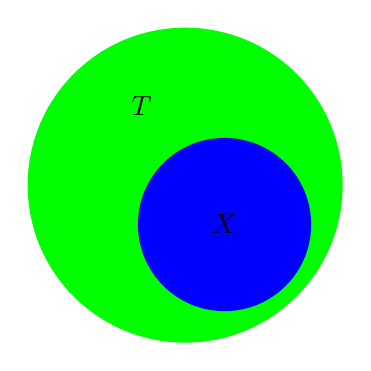
\begin{tikzpicture}
\draw [fill=green,draw=none] (-0.5,0.5) circle (2cm) node [color=black, left, xshift=-0.3cm, yshift=1cm] {$T$};
\draw [fill=blue,draw=none] (0,0) circle (1.1cm) node[color=black] {$X$};
\end{tikzpicture}
\end{center}
